\chapter{Laser operation: Continuous wave and Pulsed lasers}
\section{Continuous wave  - CW}
Consider a two mirror resonator with \textit{He:Ne} as the active medium.
The laser will run in the \textit{single model operation} with one longitudinal mode. Temporal coherence is determined by the 
resonator and not He:Ne-line width. To achieve better coherence we can decrease the cavity losses or use in-cavity spectral filtering. 
With such laser, kilo-meter long coherence lengths are achievable. One mode operation is show in figure \ref{fig:omcw}
\begin{figure}[h!]
    \centering
    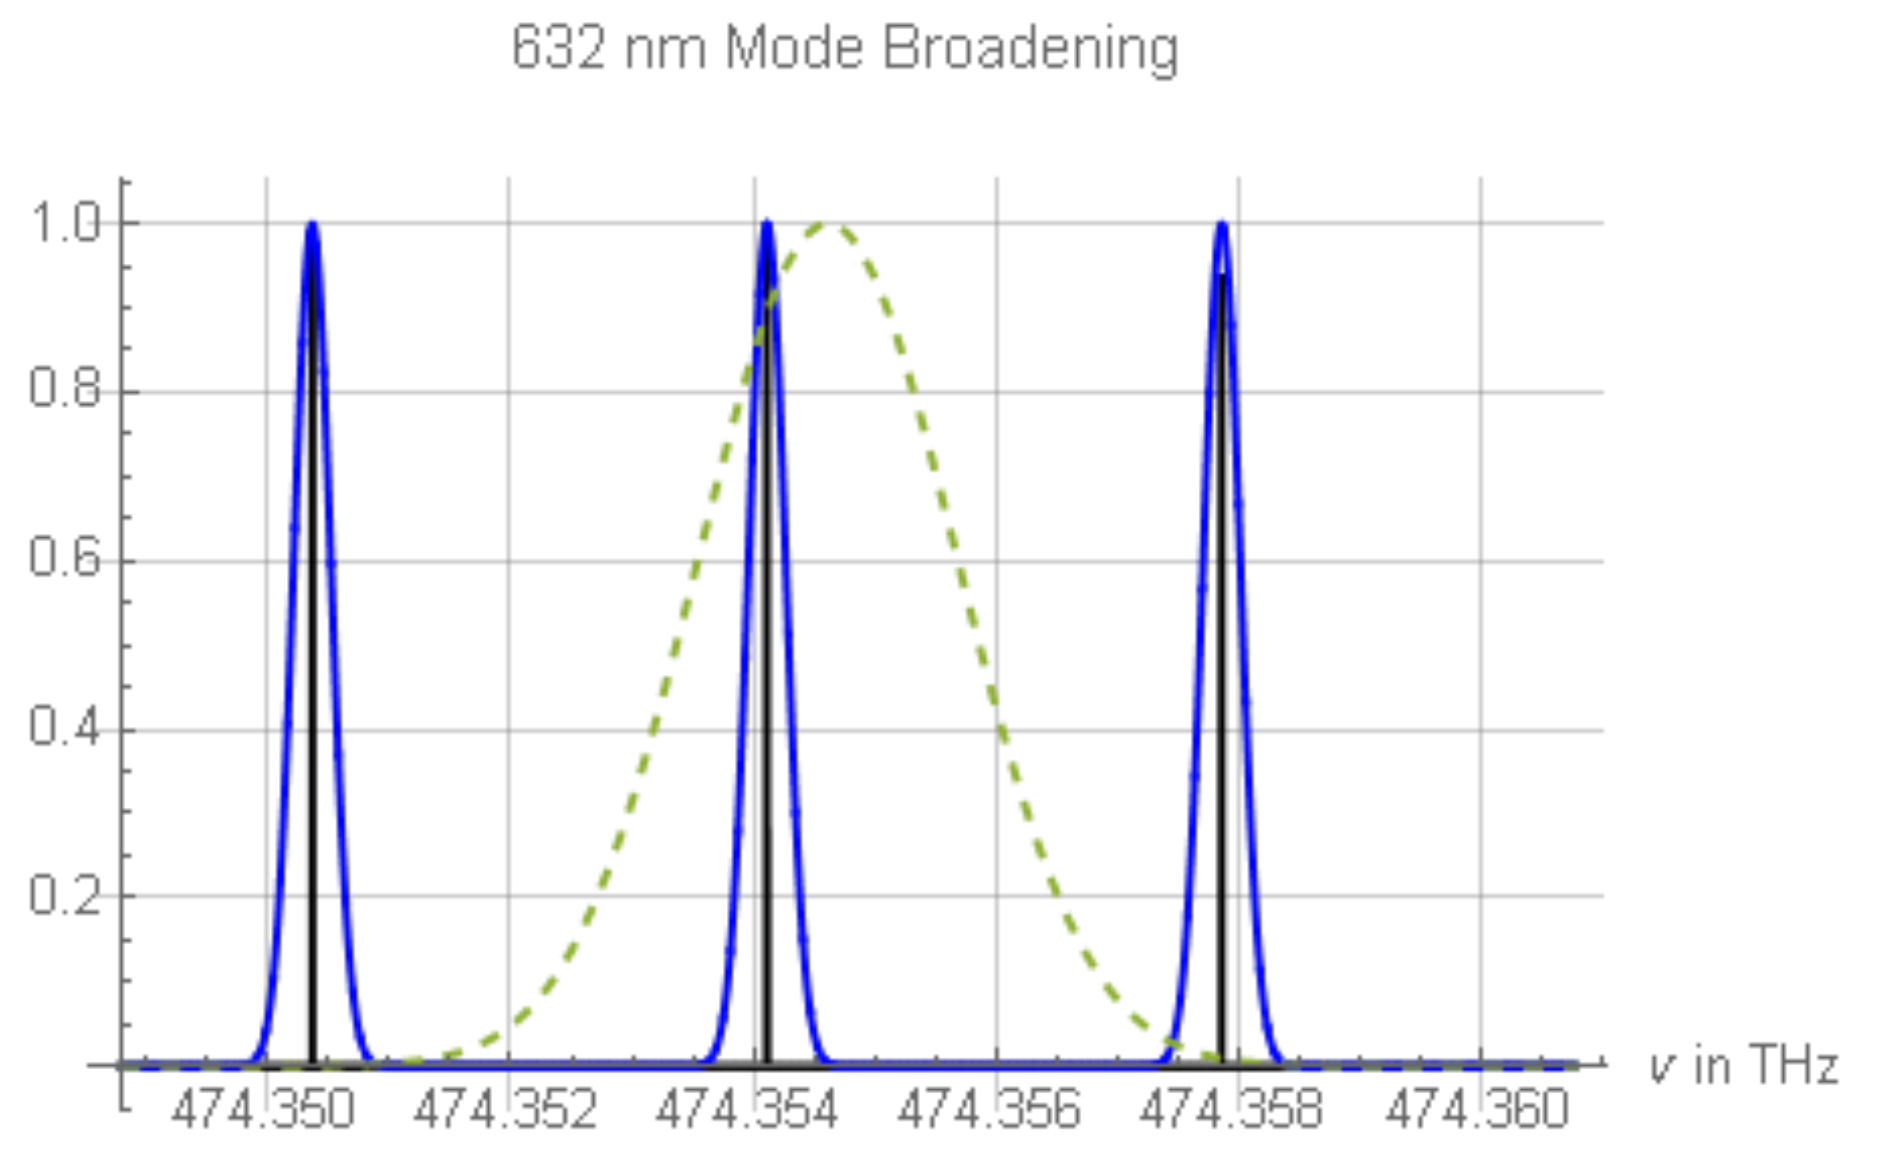
\includegraphics[width=0.5\textwidth]{slike/cw.png}
    \caption{One mode in a CW laser. \textit{Source: Lecture Notes.}}
    \label{fig:omcw}
\end{figure}

\section{Pulsed beam}
\subsection{From continuous to pulsed operation}
If the parameters of the resonator change, due to e.g. thermal expansions, vibrations \dots ,
coherence will decrease and emission frequency (wavelength) will change. Show on figure \ref{fig:hene2modes}.
\begin{figure}[h!]
    \centering
    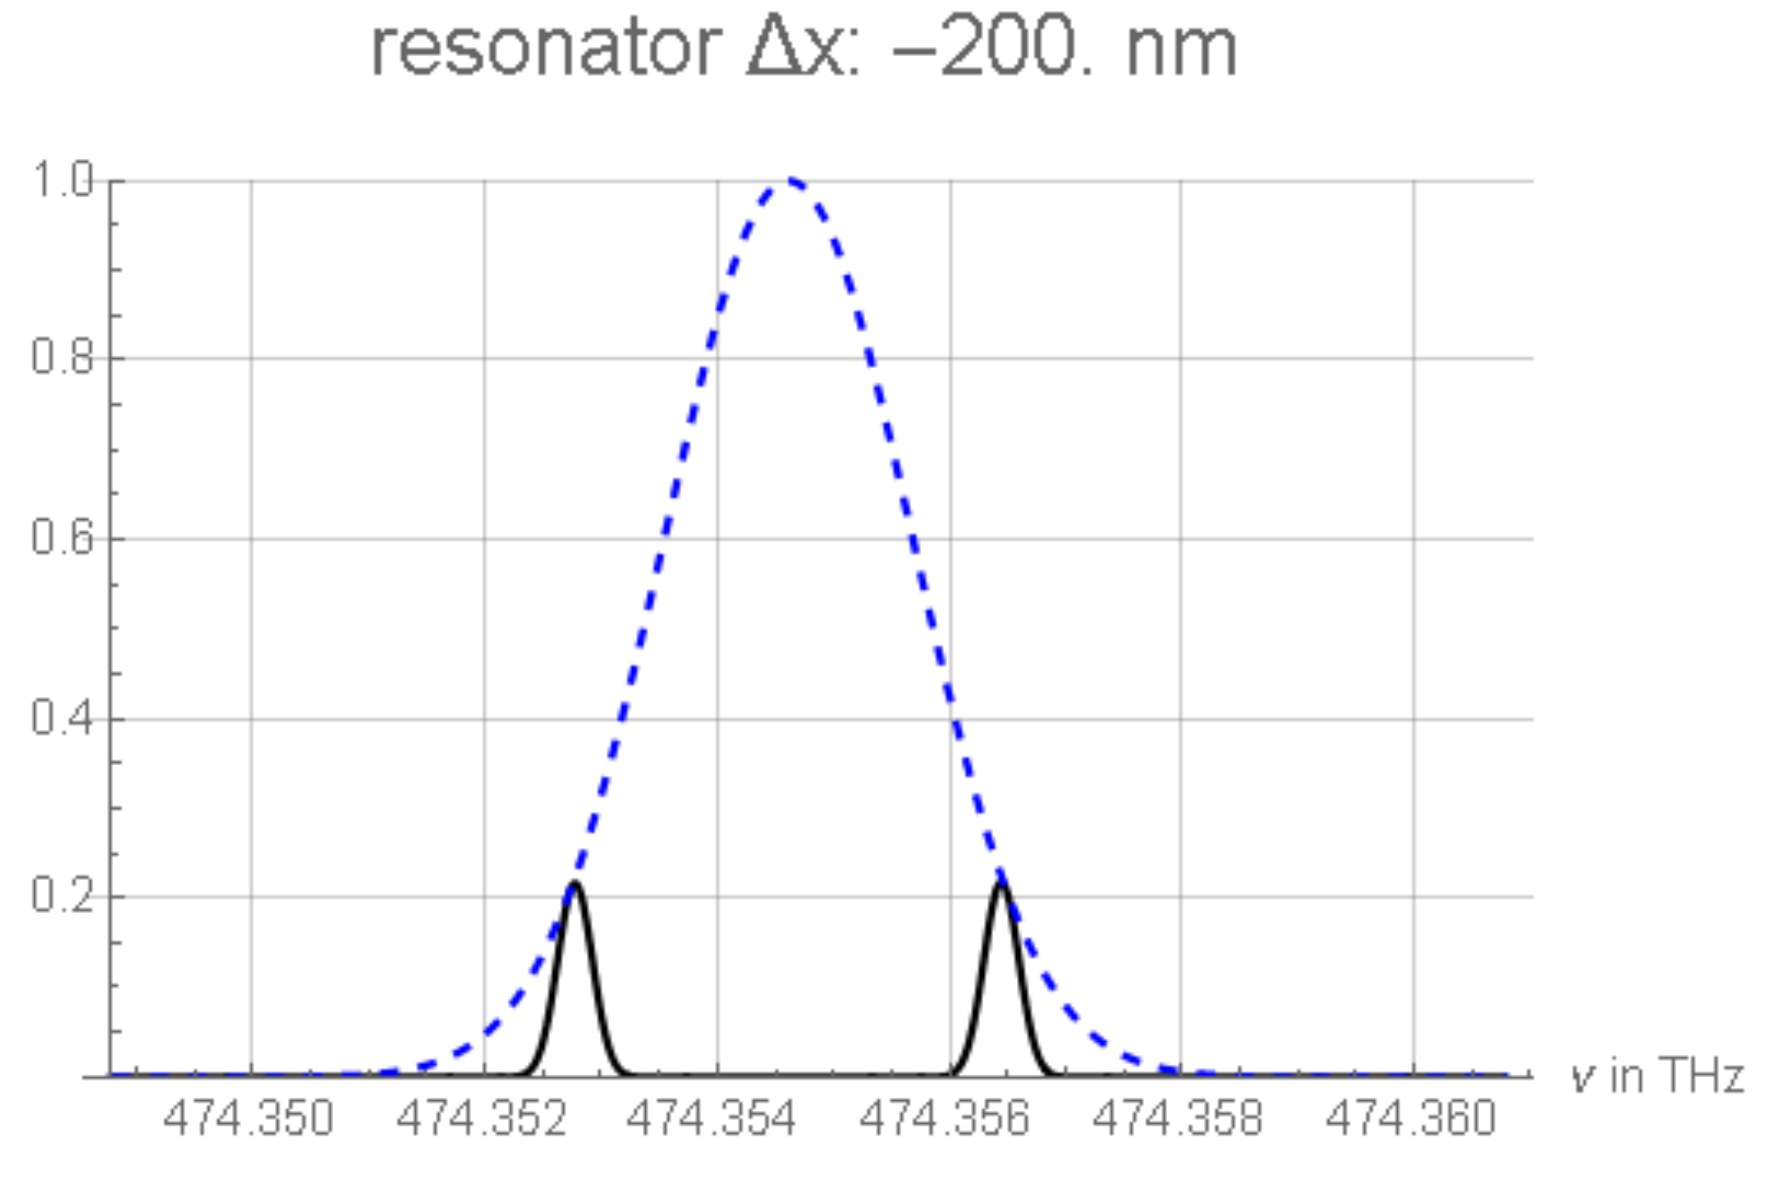
\includegraphics[width=0.5\textwidth]{slike/hene2modes.png}
    \caption{Two competing modes in the resonator. \textit{Source: Lecture Notes.}}
    \label{fig:hene2modes}
\end{figure}

Two modes will compete at constant population inversion. At first, mode $1$ will deplete population inversion until it weakens, them the second mode will rise from spontaneous emission. 
If \textbf{both modes are present at the same time}, they will \textbf{beat} - Schwebung. Beating modes are shown on figure \ref{fig:schwebung}. The beating frequency is given by the \textbf{difference} in both frequencies. 

\begin{figure}[h!]
    \centering
    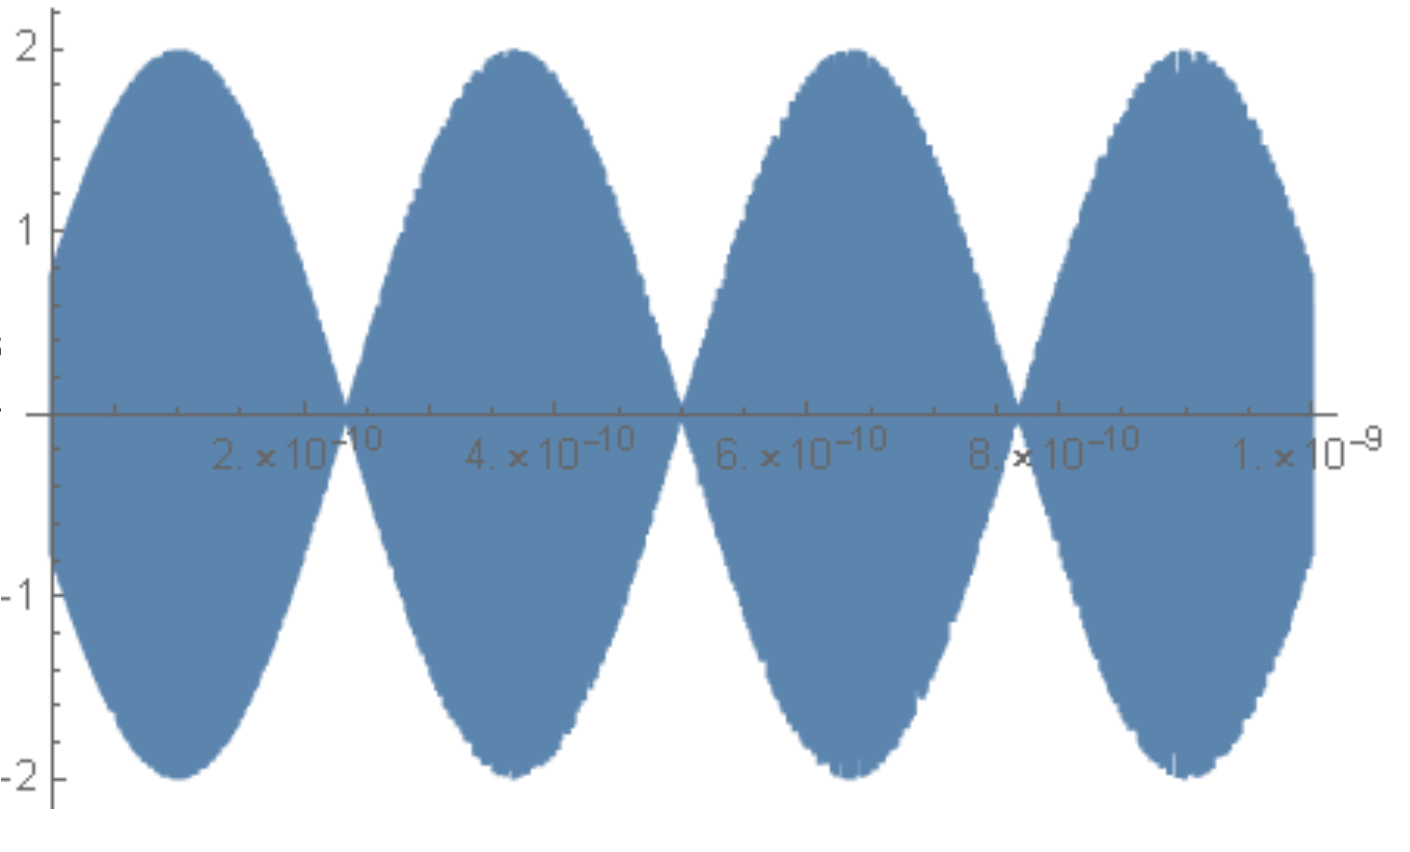
\includegraphics[width=0.5\textwidth]{slike/schwebung.png}
    \caption{Beating modes \textit{Source: Lecture Notes.}}
    \label{fig:schwebung}
\end{figure}


Laser radiation is \textbf{no longer} continuous but \textbf{pulsed}.

\subsection{Generating pulsed radiation}
To generate pulses, we can use more than just two modes, however all modes present in the resonator have to have  \textbf{locked phases} to each other.
Figure \ref{fig:mmpl} shows the output(?) of laser with 10 and 50 modes. Figure \ref{fig:mmnpl} shows the same but the phases of the modes are not locked to each other. 

\begin{figure}[h!]
    \centering
    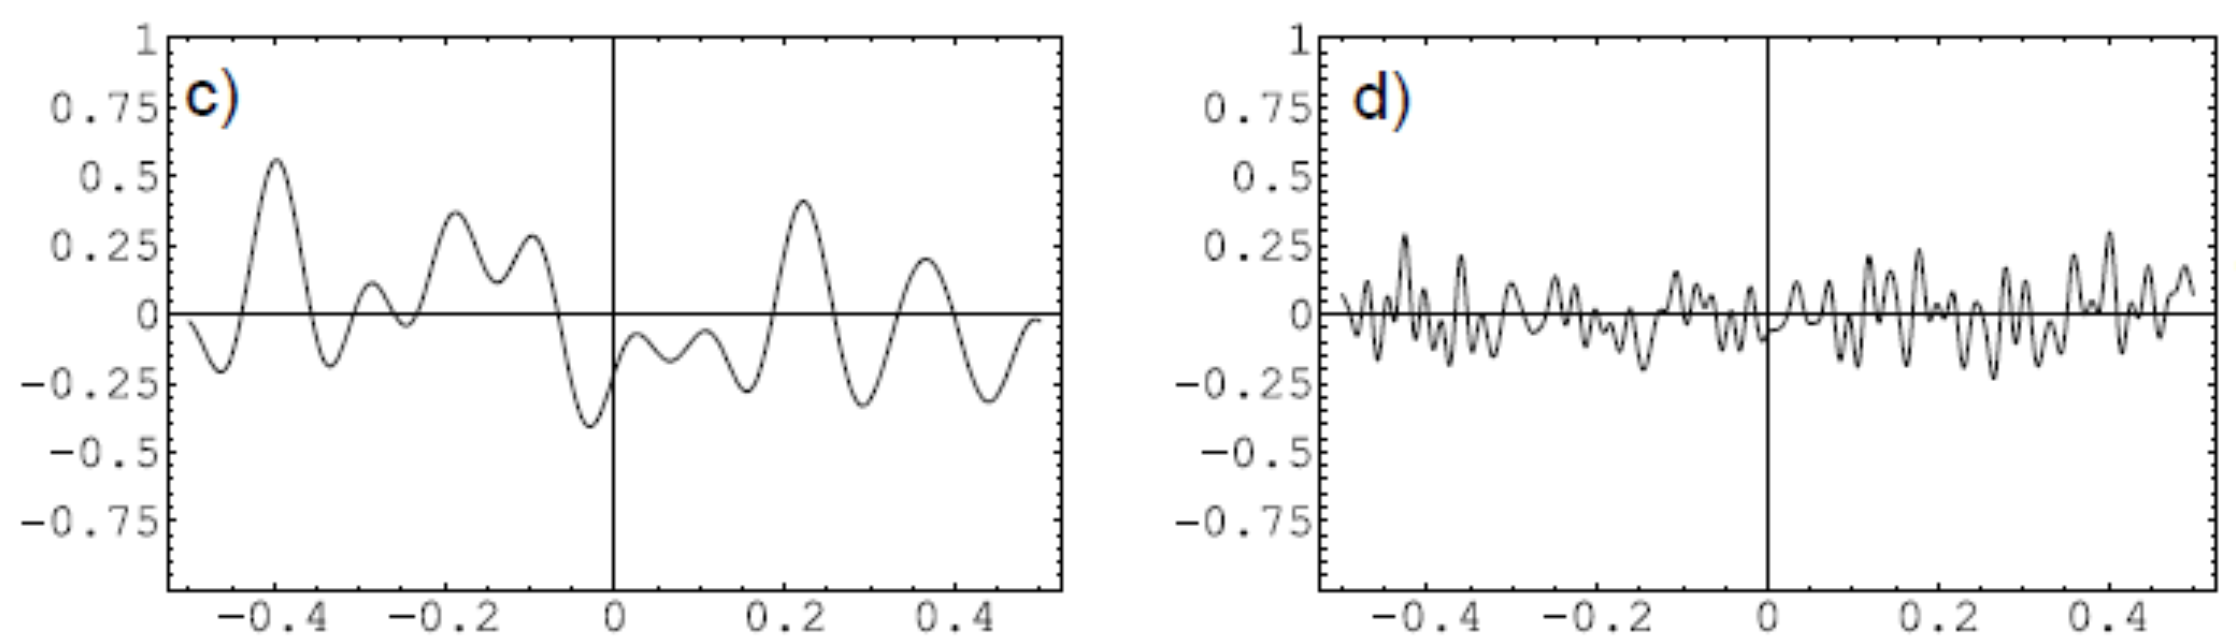
\includegraphics[width=0.75\textwidth]{slike/mmnpl.png}
    \caption{Beating modes with 10 and 50 phase locked modes. \textit{Source: Lecture Notes.}}
    \label{fig:mmpl}
\end{figure}

\begin{figure}[h!]
    \centering
    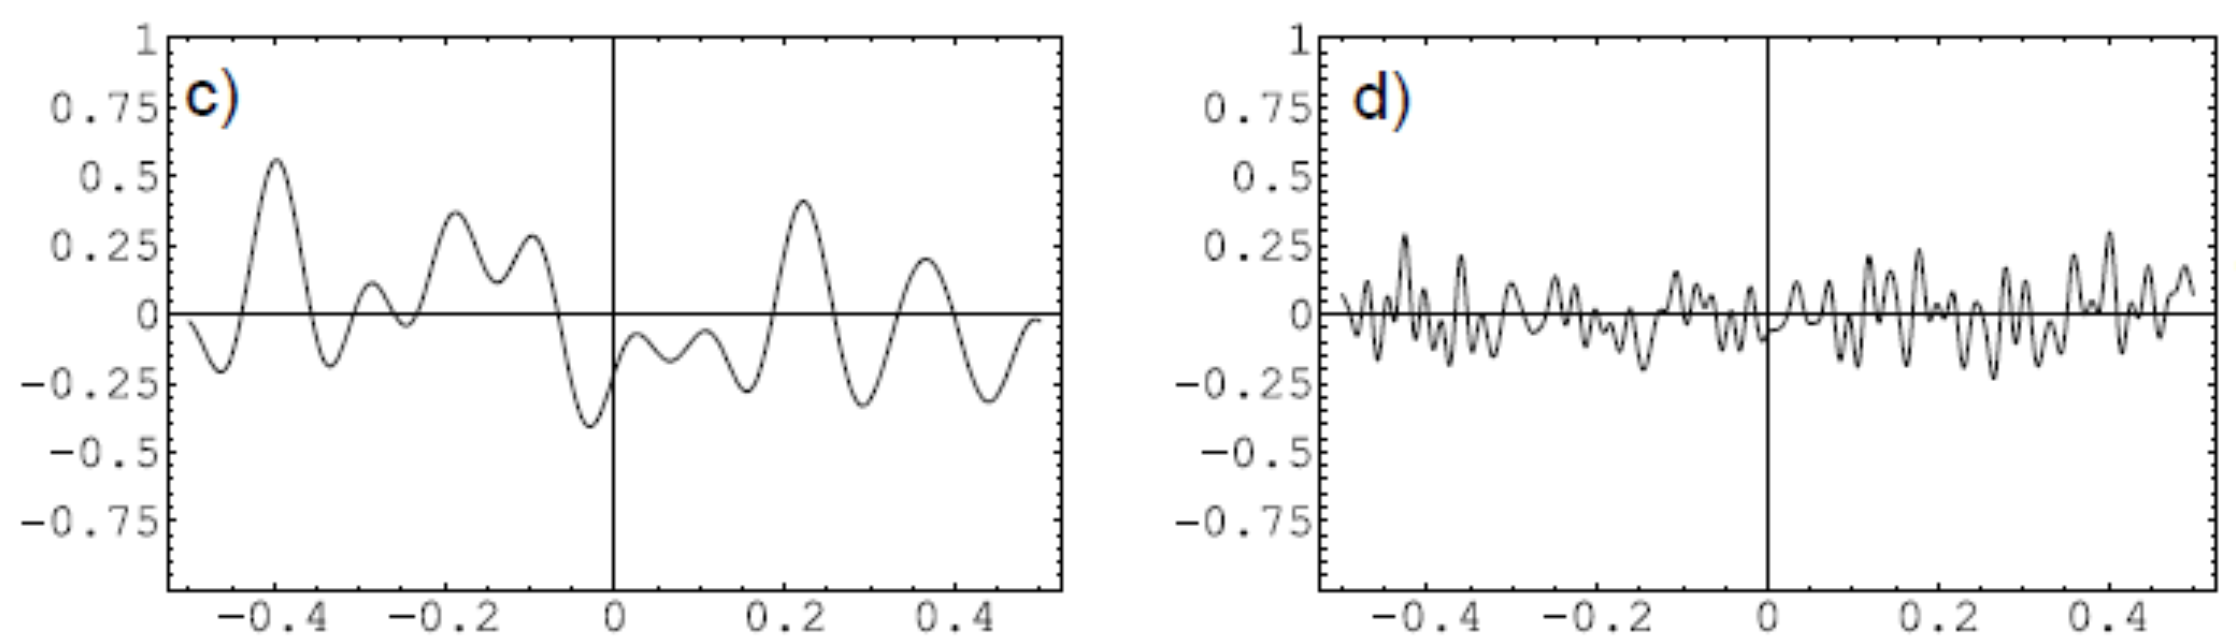
\includegraphics[width=0.75\textwidth]{slike/mmnpl.png}
    \caption{Beating modes with 10 and 50  non phase locked modes. \textit{Source: Lecture Notes.}}
    \label{fig:mmnpl}
\end{figure}

Modes with fixed phase realation, with respect to each other mode, \textbf{fully constructive interference} will only be possible at \textbf{one point in time}, everywhere else interference is destructive. 
Show in figure \ref{fig:mmif}.
\begin{figure}[h!]
    \centering
    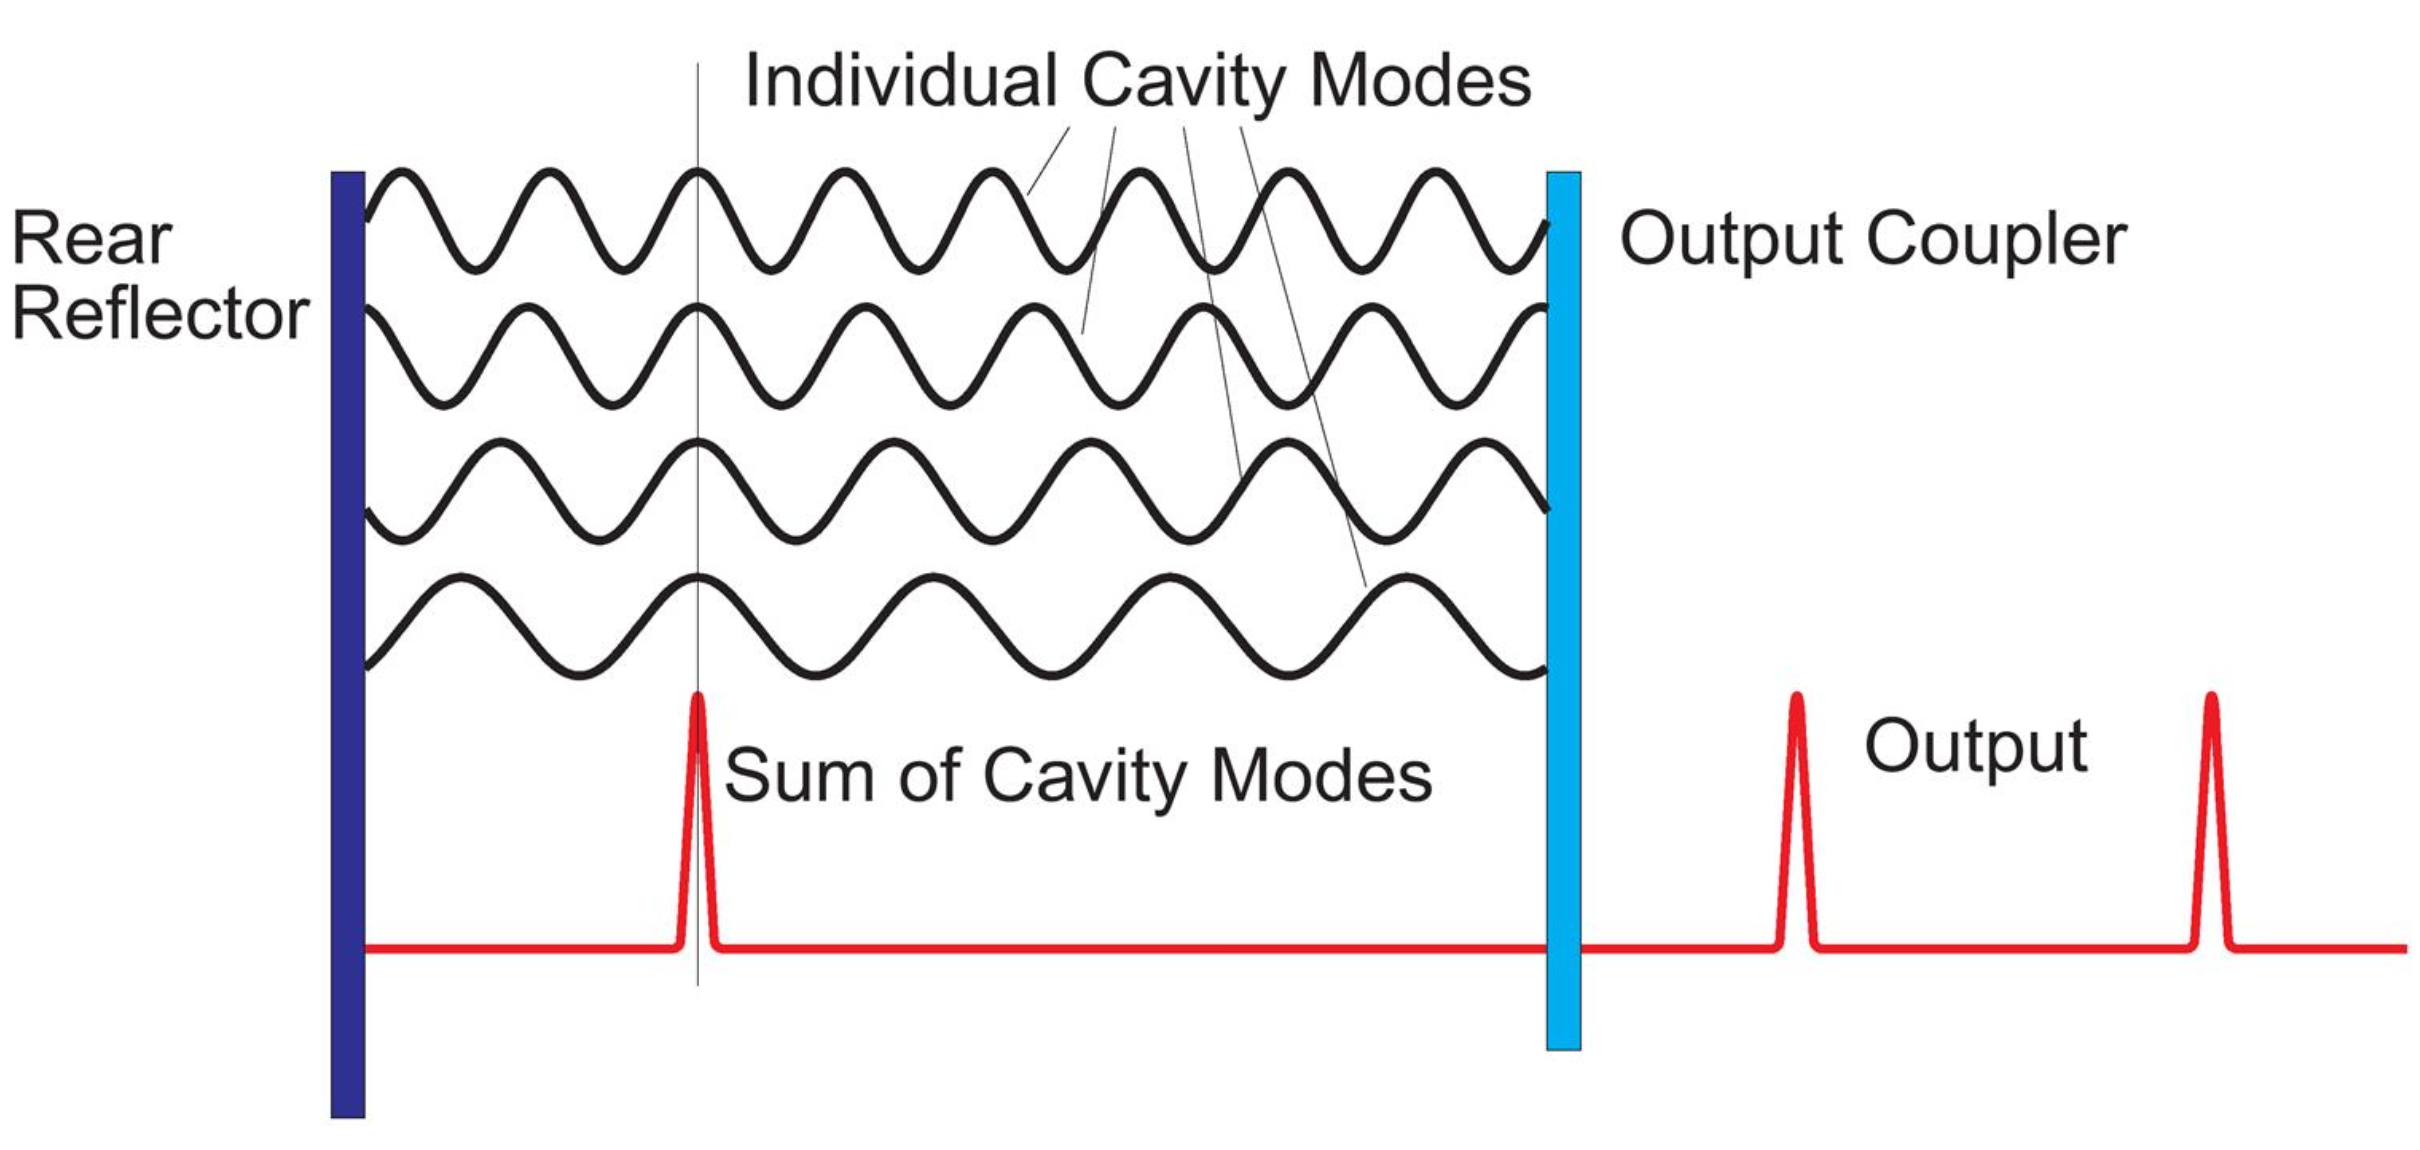
\includegraphics[width=0.5\textwidth]{slike/mmif.png}
    \caption{Interference in a resonator with multiple modes. \textit{Source: Lecture Notes.}}
    \label{fig:mmif}
\end{figure}


\section{Generating pulsed radiation}
\subsection{Mode locking}

Starting from a single CW-mode we can create new modes with external modulation. Shown on figure \ref{fig:em1}.
\begin{figure}[h!]
    \centering
    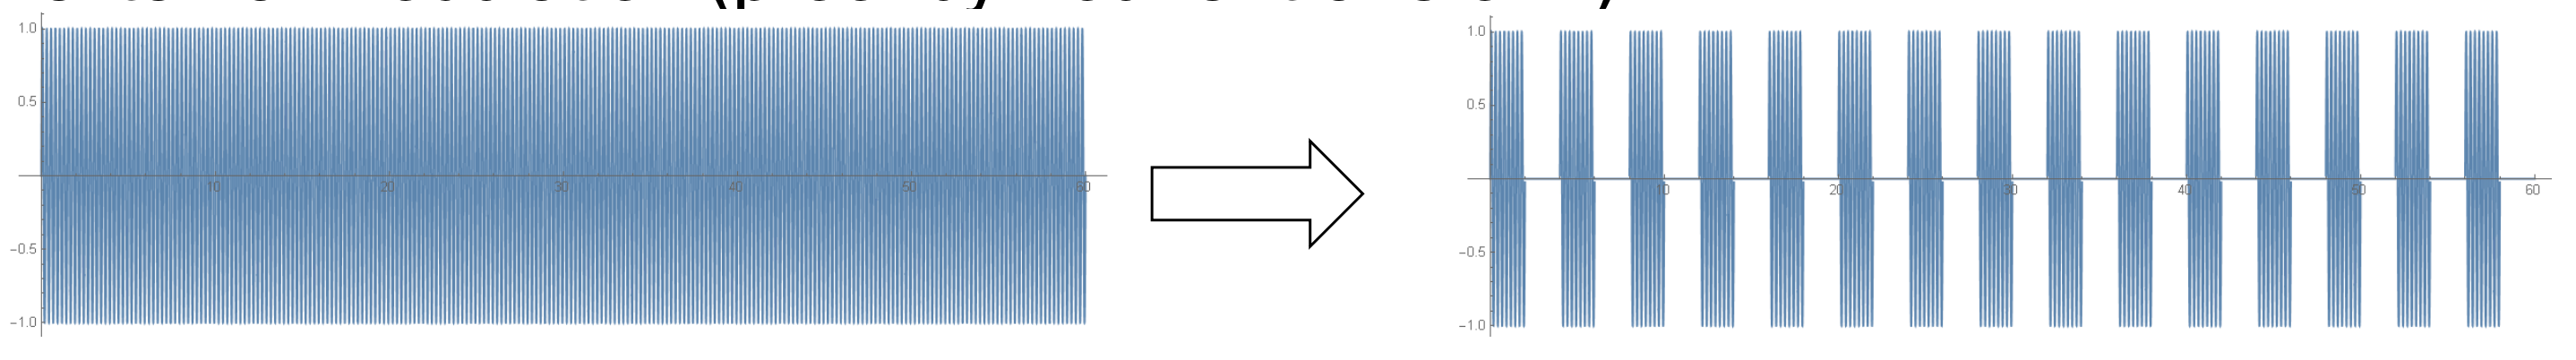
\includegraphics[width=0.75\textwidth]{slike/em1.png}
    \caption{Single to multimode conversion  with external modulation. \textit{Source: Lecture Notes.}}
    \label{fig:em1}
\end{figure}

(External) modulation redistributes the energy from the main frequency peak to the side bands, which were not present with single mode operation.
Frequency spacing of the side-bands depends on modulation frequency. Due to the phase relation to the main wave side-bands have fixed periodic modulation. 
Fourier transform \textit{keeps} the phase information. Figure \ref{fig:em2} shows the FT after external modulation.

%maybe redraw?
\begin{figure}[h!]
    \centering
    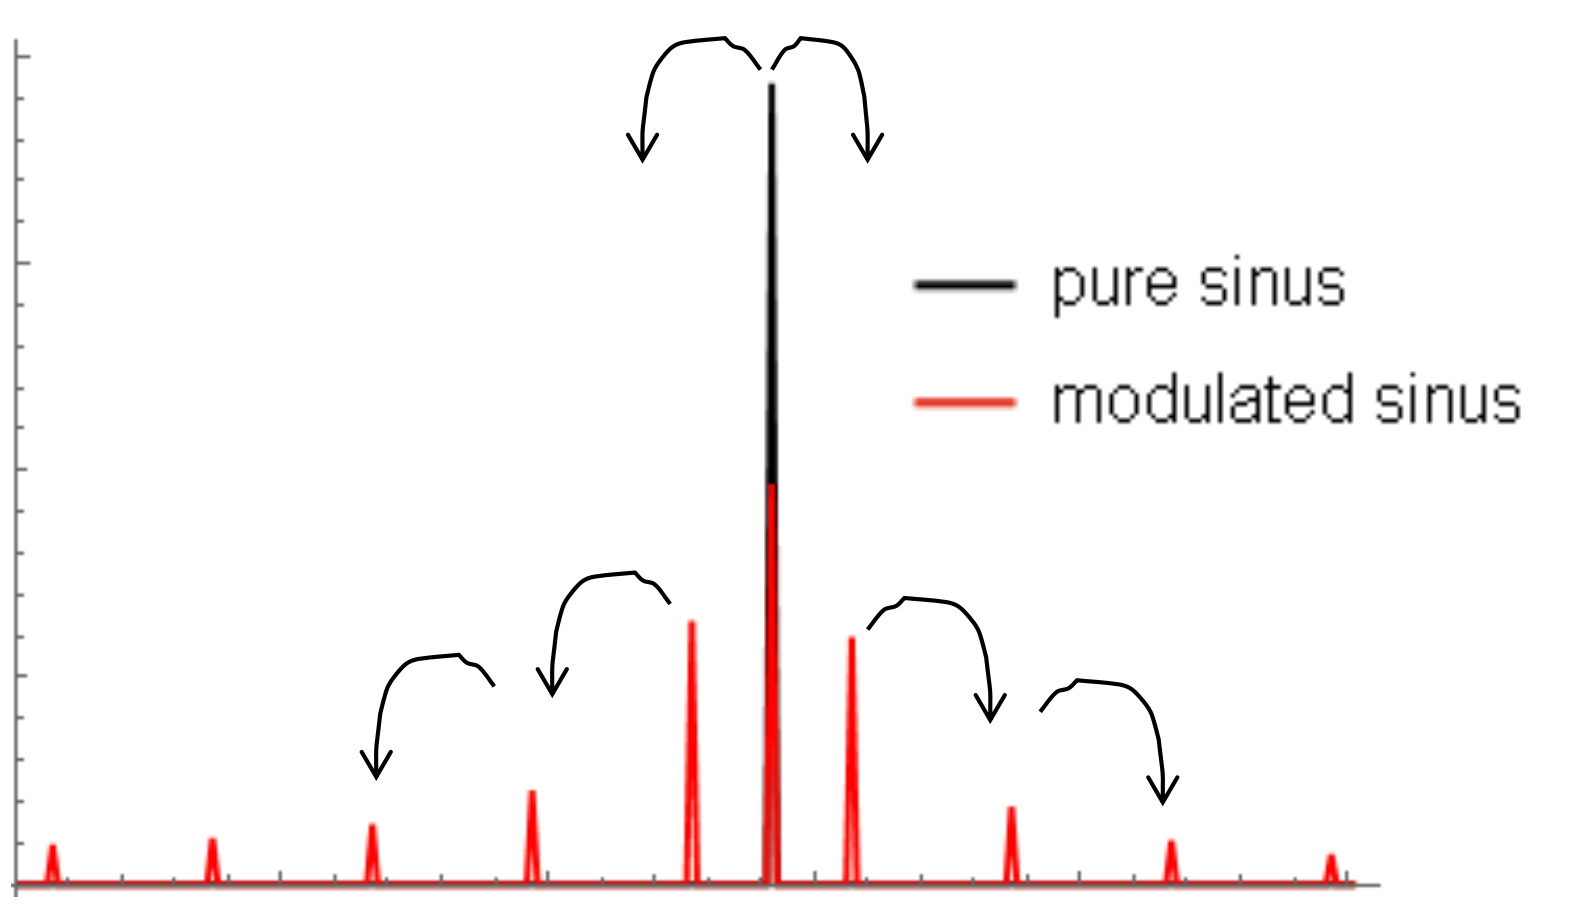
\includegraphics[width=0.5\textwidth]{slike/em2.png}
    \caption{FT of external modulation. \textit{Source: Lecture Notes.}}
    \label{fig:em2}
\end{figure}

If we modulate with a frequency that coincides with the longitudinal modes of the resonator and the laser can emit light at that frequency. Light with the side band's frequencies \textbf{will exist in the resonator}.

If the sidebands coincide with longitudinal resonator models, pulse generation is possible even if only one
mode is available.  If the laser medium supports only one mode stimulated emission is only available for that mode, all
other modes decay. Their lifetime depends on resonator quality and efficiency of modulation.

If the gain medium supports several modes, mode locking \textbf{will transfer energy} between modes, while generating additional sidebands.
Phases of the modes will become synchronized over time, because sidebands generated by modulation  have a phase fixed to the main wave and
phase locked wave "wins the competition" for population inversion after some time - compared to the wave with same $\nu$ but random phase.

\subsubsection{Passive mode locking}
For \textbf{active} mode locking, we only considered active modulation - controlling the external light modulation.

For \textbf{passive} mode locking mechanisms, we can use \textbf{non-linear} materials with \textit{intensity} dependent properties.
Using such materials high intensity experiences smaller losses/absorption or higher reflectivity. Non-linear materials are $Er^{+3}$ glass (non-linear absorption), sapphire (non-linear refraction),
air (non-linear refraction), glass (non-linear refraction) and SESAM (non-linear reflection).

\textit{Note: Linear behaviour is considered as the standard. For linear materials properties such as reflectivity, absorption, speed of propagation are constant.}

\subsection{Kerr-lens mode-locking}
Kerr-lens is an effect, which causes the index of refraction to change at higher laser intensity.
At high intensity index of refraction  is $n = n(\lambda) + n_2 \cdot I$, where $n_2$ is the non-linear \textit{constant} index of refracion.
It is very small, $~10^{-16} \frac{cm^2}{W}$, so the non-linear effect is only important at high peak laser power $~P > 1MW$.
Kerr-Effect is shown on figure \ref{fig:kerreff}.

\begin{figure}
    \centering
    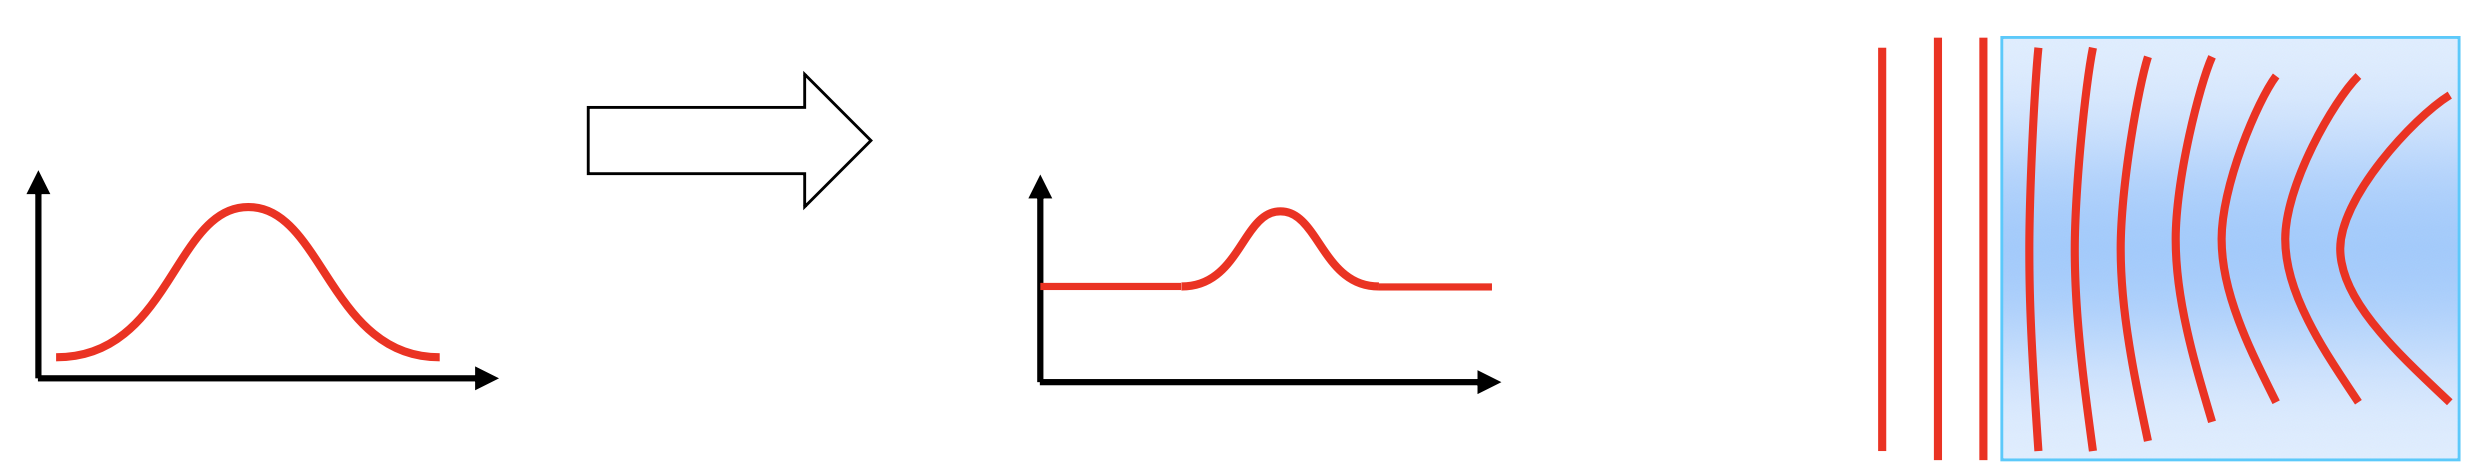
\includegraphics[width=0.75\textwidth]{slike/kerreff.pdf}
    \caption{Kerr effect \textit{Source: Lecture Notes.}}
    \label{fig:kerreff}
\end{figure}


Kerr-lens mode-locking is a form of passive mode-locking, which generates short pulses using a lens.
\textbf{Kerr-lens} mode locking is only present at high intensities. Strength of the Kerr-lens effect depends on the intensity.
Changes of refractive index change occurs at the time scales of $~1 fs$, which is about equal to the roundtrip of an electron on
its orbital. Intensity fluctuations are the result of \textbf{very low coherence} in of the laser. Lower coherence means sharper peaks in intensity. 
Each sudden peak in intensity will experience a small lensing effect in the resonator. 

We wish to build a resonator, which is more stable or has lower losses in if there is a lens present in the active medium.
We can dampen the lower intensity modes using an \textbf{aperture}, but it is not always needed. Higher intensities will have gain higher than low intensities - 
lower intensities will grow weaker, while the  higher intensity modes will grow stronger. 
During each roundtrip the high peak power will modulate the transmissivity of the laser medium and resonator system periodically.
Mode locking and power transfer occurs between many modes.

\subsection{Semiconductor Saturable Absorber Mirror - SESAM}
Using a SESAM materials is another option to dampen the low intensity modes. SESAM is an optical element, which 
absorbs low intensities, but becomes saturated at a certain threshold and becomes reflective. Lower intensities, which were absorbed, can
not propagate in the resonator. 

\textbf{SESAM} is constructed form two components - a \textit{Bragg-Mirror} with a 
saturable absorber in front, shown in figure \ref{fig:sesam}.

\begin{figure}[h!]
    \centering
    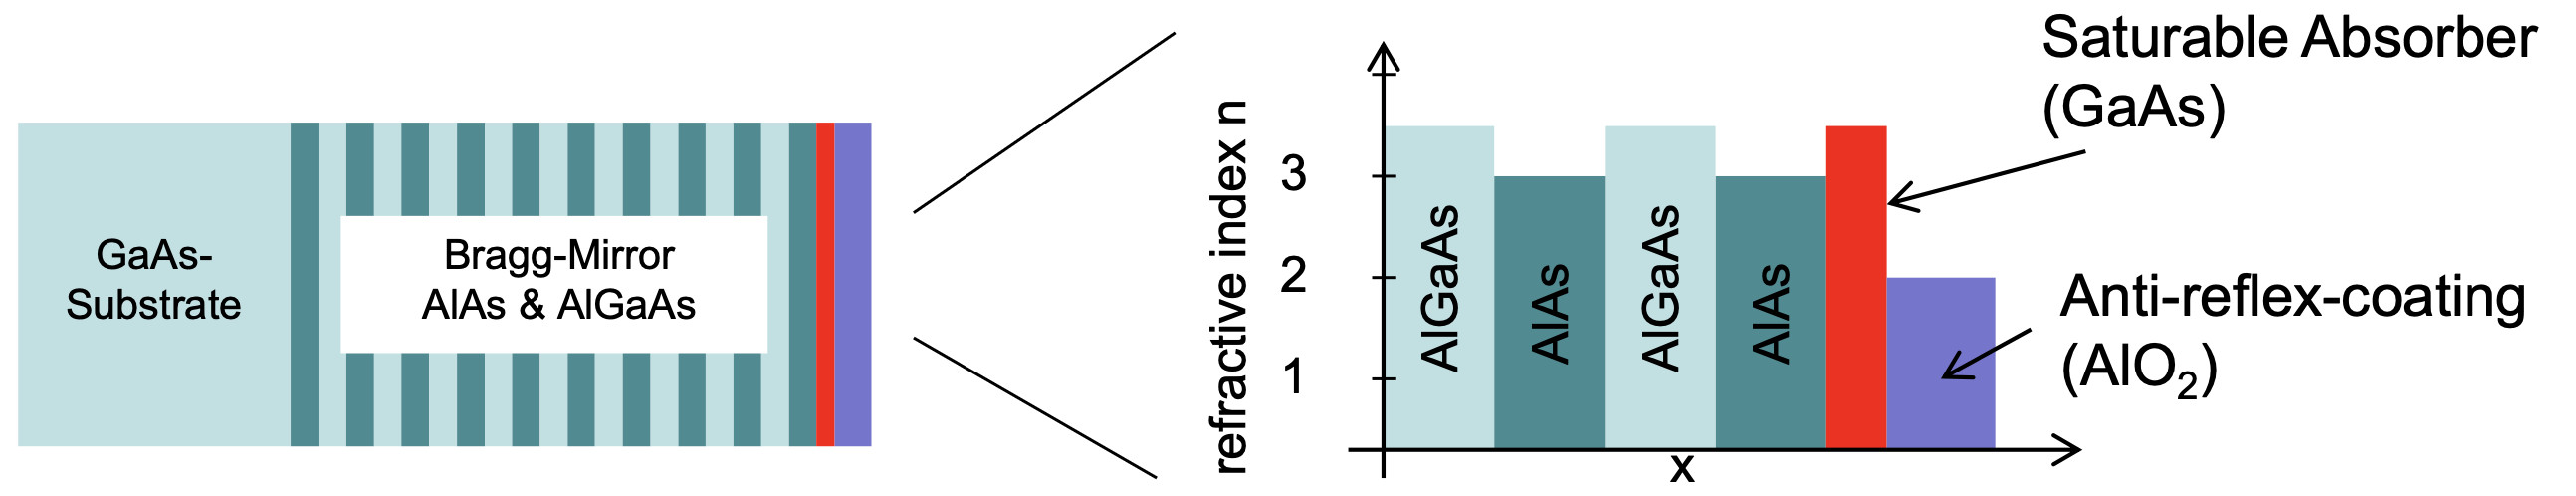
\includegraphics[width=0.75\textwidth]{slike/sesam.png}
    \caption{SESAM \textit{Source: Lecture Notes.}}
    \label{fig:sesam}
\end{figure}

At low intensities the absorber will generate an electron-hole pair, at high enough intensity the materials is saturated. 
No further pairs can be created - light is transmitted and reflected at the Bragg mirror. After some time, the electron-hole pairs
recombine - shown on figure \ref{fig:sesam2}.
\begin{figure}[h!]
    \centering
    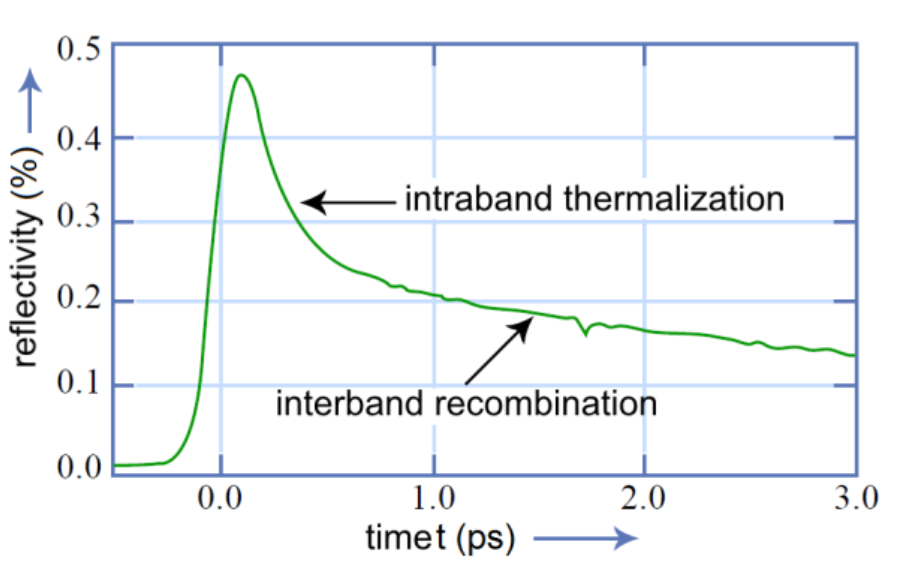
\includegraphics[width=0.35\textwidth]{slike/sesam2.png}
    \caption{Working of SESAM. \textit{Source: Lecture Notes.}}
    \label{fig:sesam2}
\end{figure}

\subsection{Q-Switching}

Figure \ref{fig:qswitching} shows a laser resonator with quality switching (Q-switch).
\begin{figure}[h!]
    \centering
    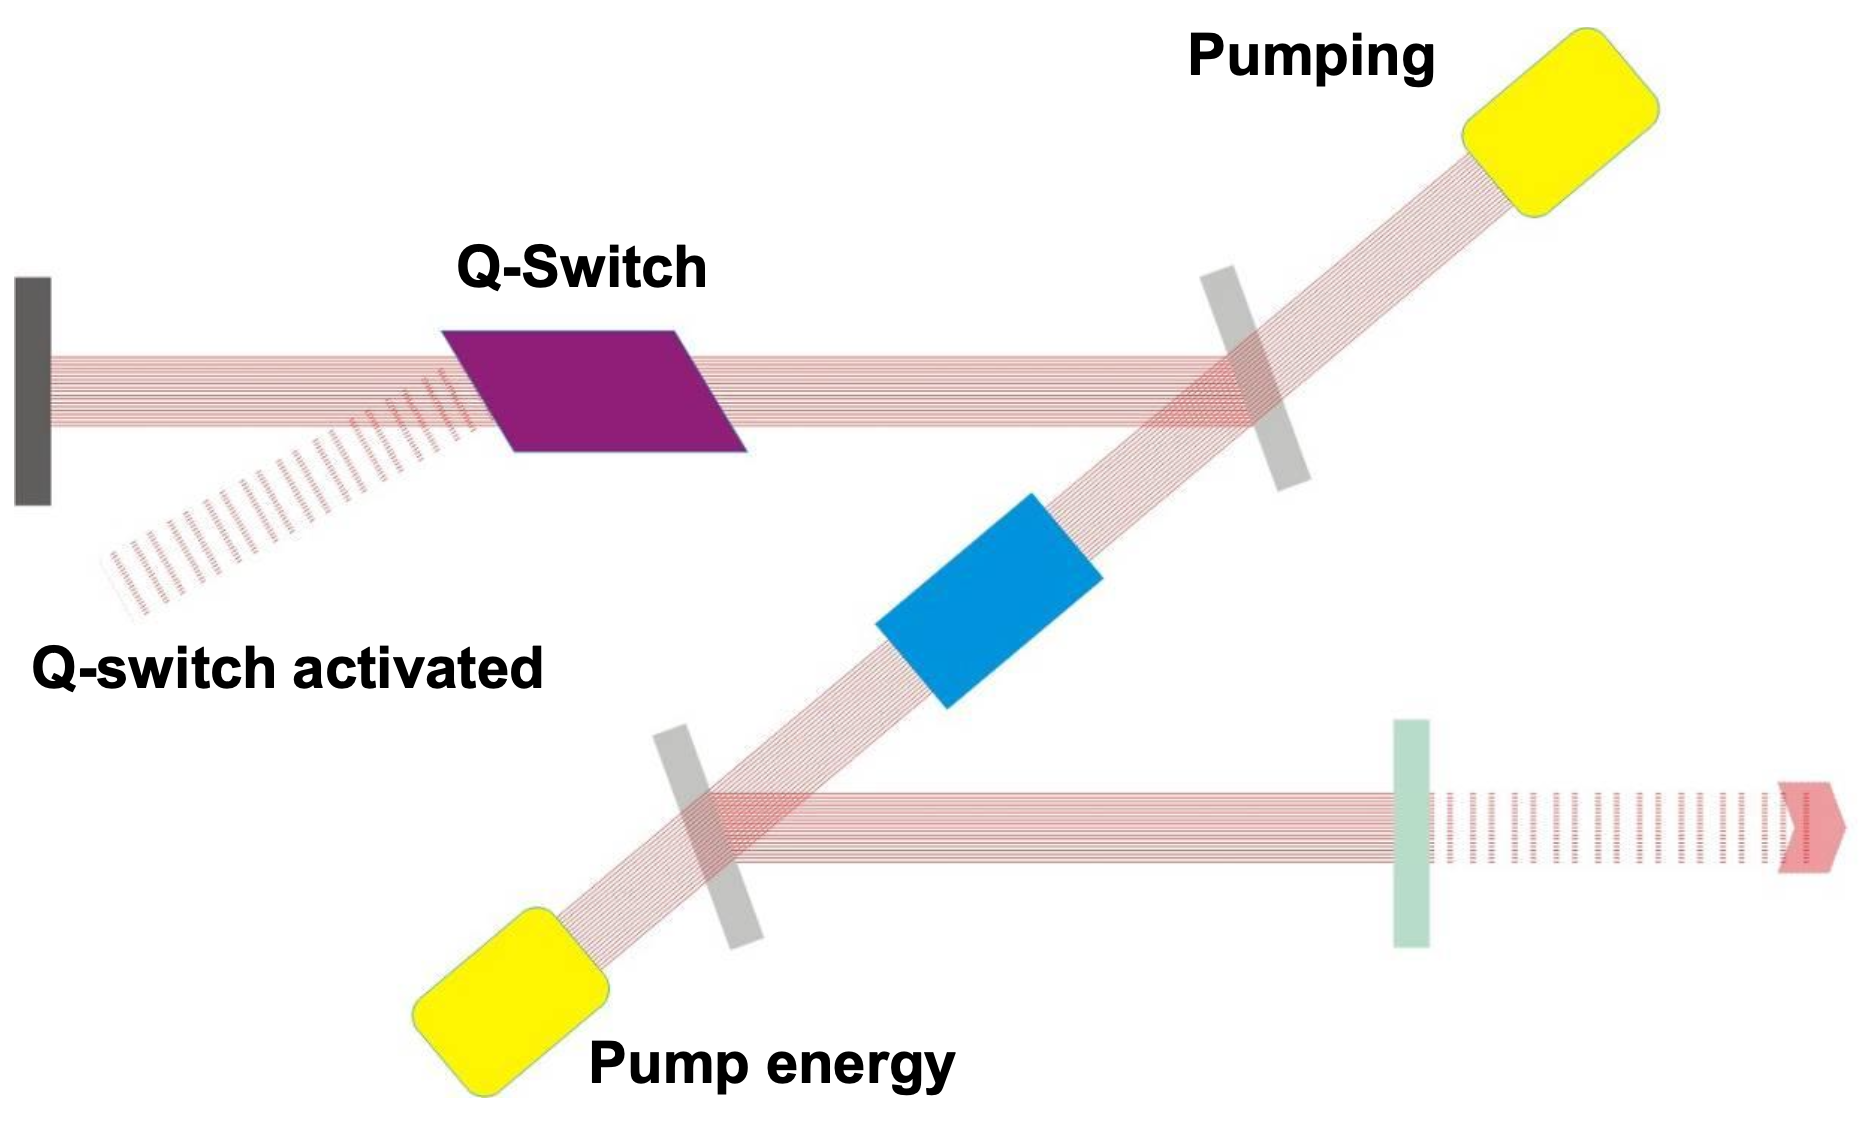
\includegraphics[width=0.5\textwidth]{slike/qswitching.png}
    \caption{Laser resonator with Q-Switching. \textit{Source: Lecture Notes.}}
    \label{fig:qswitching}
\end{figure}

When the Q-switch is activated, there is no laser emission, population is building up but the losses in the resonator are high.
When the Q-switch is deactivated the laser emits a high energy pulse. Typical pulse duration is 1 to 500 ns. 
The pulse from a Q-switched laser is longer (compared to mode locking) but it enables higher control of pulse generation.
